\chapter{État de l'art}
\label{2_state_of_the_art}


\section{\textit{Smart Cities}}

Les Smart Cities, également connues sous le terme villes intelligentes, sont des villes qui utilisent des technologies de l'information et de la communication afin d'améliorer les services urbains en faveur des citoyens \cite{Smartcit54:online}. Pour cela, ces villes utilisent un large panel de capteurs qui ont pour but d'acquérir des données afin d'améliorer la gestion des ressources et des actifs. De plus en plus de ces villes offres des flux de données en temps réel pour informer les déplacements de ses citoyens. La gestion des feux automatiques afin d'optimiser les déplacements des automobilistes et ainsi réduire les ralentissements du réseau routier en son un exemple. \\


Aux États-Unis, en 2017, 66\,\% des villes ont investis dans les technologies liées aux Smart Cities \cite{66ofUSci17:online} selon une étude de la \textit{National League of Cities} (NLC). Et parmi les 34\,\% restants, 25\,\% sont actuellement en train d'explorer les différentes possibilités d'investissement. La NLC indique que les principaux domaines connectés sont : 

\begin{itemize}
    \item les compteurs intelligents pour les services publics;
    \item les signaux de trafic intelligents;
    \item les applications de gouvernance électroniques;
    \item les kiosques Wi-Fi;
    \item les capteurs d'identification par radiofréquence (RFID) dans la chaussée.\\
\end{itemize}

Selon le rapport \textit{Smart Cities Market} par Focus Area, le marché des Smart Cities se montera à 1 201,69 milliards USD en 2022 avec un taux de croissance annuel de 23.1\,\% entre 2017 et 2022 \cite{SmartCit61:online}. Ceci montre bien qu'il s'agit là d'un marché en plein développement qui attire beaucoup d'investisseurs. Toutes ces technologies doivent se baser sur des plateformes communes, afin d'éviter la fragmentation des données. Le véritable \textit{challenge} réside justement sur cette plateforme qui doit être pensée afin d'être générique sans ajouter une trop grande complexité pour les différents partenaires. Il y a également la problématique des flux de données, car certains capteurs génèrent de grands flux de données (ex. capteurs en temps réel) alors que certains n'effectuent qu'une à deux mesures journalières. Ce sont donc deux types de capteurs ayant des besoins bien différents, que ce soit en termes de consommations ou de débit de données. L'une des raisons pour lesquels ces plateformes doivent accepter plusieurs protocoles en fonctions des différents besoins.\\

De plus en plus de villes, à l'image de celles des États-Unis, sont intéressées par ces nouvelles opportunités et Genève n'est pas en reste. En effet, Genève met déjà à dispositions de ses citoyens, ainsi que des entreprises, plusieurs données publiques. Une partie de ces données sont disponibles sur le portail du SITG\footnote{Système d'information du territoire à Genève (SITG) \url{http://ge.ch/sitg/}} sous forme de cartes interactives. La \cref{fig-sitg_mobilite} contient un visuel sur l'état des différents axes routiers à l'aide du portail du SITG. D'ici 2030, le canton de Genève s'est donné pour objectif stratégique de devenir un pilier dans le domaine des Smart Cities \cite{Genevebr38:online} en développant de nouveaux projets et services autour de cette thématique.

\begin{figure}[ht!]
    \centering
    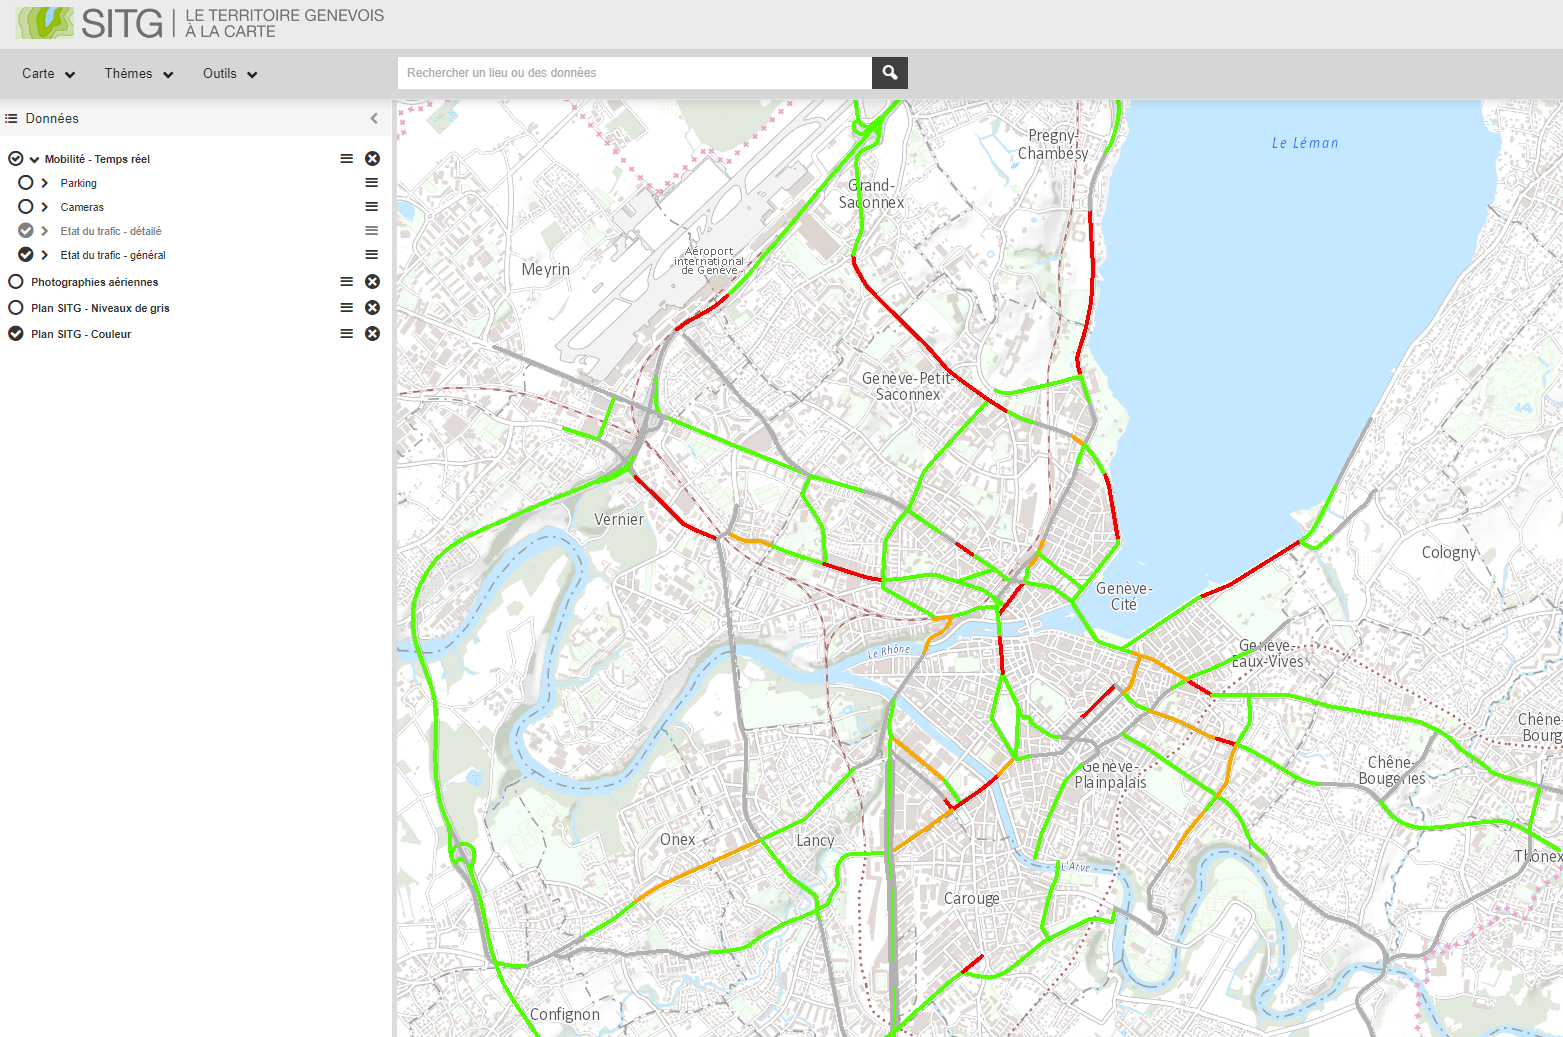
\includegraphics[width=0.80\textwidth]{Figures/StateOfTheArt/sitg_mobilite.PNG}
    \caption{Carte du trafic des principaux axes routiers de Genève en temps réel sur le portail SITG}
    \label{fig-sitg_mobilite}
\end{figure}


En Suisse, il existe une initiative de l’Office fédéral de l’énergie et de SuisseEnergie nommée Smart City Suisse \cite{SmartCitSuisse:online}. Il s'agit d'un programme ayant pour but de créer une plateforme d'information et d'échange pour les différentes villes de Suisse. Cette initiative est 
destinée aux communes qui souhaite planifier leur avenir afin d'accroitre leur statut de \textit{Smart City} à l'aide de différents partenaires. Le programme se considère comme plateforme d’information et d’échange. À l'heure actuelle, cette plateforme a déjà aidé plus de 200 projets\footnote{\url{http://ds1.dreifels.ch/smartcity/wprlist.aspx?LA=de}} à se développer en Suisse et en Europe dans le but d'améliorer la qualité de vie dans diverses villes. Les projets sont divisés en 10 thématiques, allant de la gestion de l'énergie à la santé, en passant par l'éducation et la sécurité.\\

Genève a annoncé, dans le cadre de son projet de SmartCanton \cite{LeTempParkings:online}, l'installation de capteurs sur 650 places de parkings. L'objectif de cette installation est de connaitre en temps réel l'occupation de ces places de stationnement dans le but d'informer les automobilistes des cases libres, mais également de faciliter le paiement du temps de stationnement. Le conducteur est guider à l'aide de panneaux de guidage dynamique ou d'une application smartphone \cite{LeTempParkings:online}. En 2015, un premier projet pilote a été mis en place dans la commune de Carouge en utilisant des capteurs développés par l'entreprise genevoise IEM\footnote{\url{http://www.iemgroup.com/fr/solutions-produits/capteurs/presto-sense/}}. 

\section{LPWAN}
\label{sec-stateOfTheArt_LPWAN}

Les réseaux \textit{Low-Power Wide-Area Network} (LPWAN) sont des réseaux qui sont de nos jours en pleine expansion, en partie grâce à la croissance des villes intelligentes \cite{LPWANWik63:online}. Le placement des LPWAN à comparer aux différentes technologies sans fils est visible sur la \cref{fig-lpwan_vs_others} \cite{LPWANisL94:online}. On peut constater que les LPWAN s'associent bien avec les technologies existantes, en comblant des vides laissés par celles-ci. Les débits disponibles sur les LPWAN oscillent entre 0.3 kb/s et 50 kb/s \cite{1607080117:online}. Cela limite donc drastiquement les domaines d'application des capteurs qui peuvent utiliser ces technologies. Le débit de ces capteurs est restreint, mais les LPWAN sont surtout attractifs pour leur portée, et donne la possibilité de créer des périphériques de basse consommation, avec un faible cout unitaire. L'autonomie des dispositifs LPWAN peut atteindre plusieurs années en fonction de la fréquence des paquets envoyés et la taille de la batterie utilisée.

\begin{figure}[ht!]
    \centering
    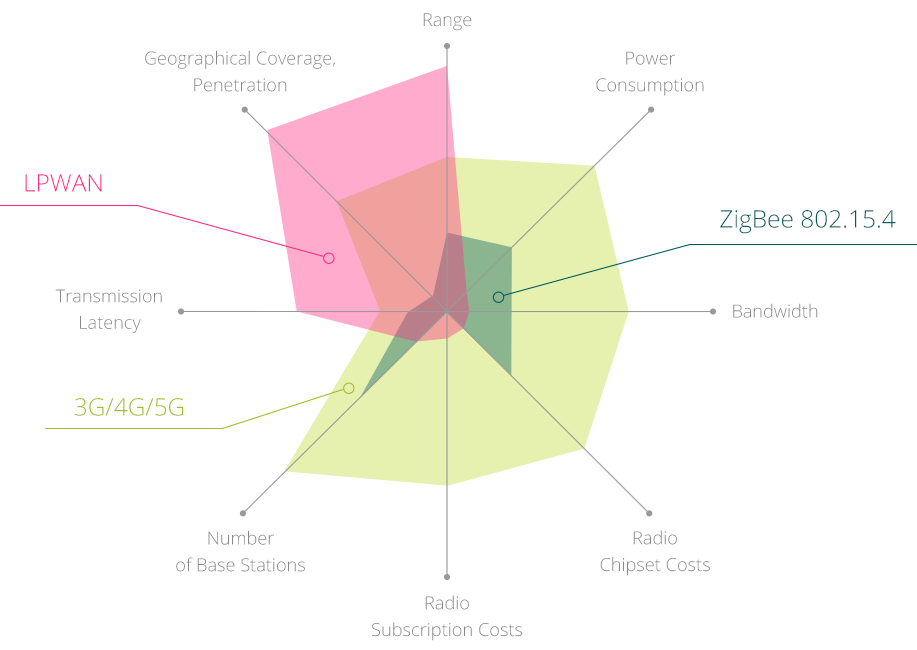
\includegraphics[width=0.75\textwidth]{Figures/StateOfTheArt/lpwan_vs_others.png}
    \caption{Comparaison de LPWAN avec d'autres technologies}
    \label{fig-lpwan_vs_others}
\end{figure}

Il existe principalement deux types de technologies sur lesquels se base les différents protocoles :
\begin{enumerate}
    \item LoRa : LoRa est une modulation radio utilisée par plusieurs protocoles tels que LoRaWAN\footnote{\url{https://www.lora-alliance.org/technology}}, Haystack Technologies\footnote{\url{http://haystacktechnologies.com/}} ou encore Symphony Link \footnote{\url{https://www.link-labs.com/symphony}} \cite{LPWANWik63:online}. Cette modulation est la propriété du fabricant de semiconducteurs Semtech depuis 2012. Elle est principalement présente dans la gamme de fréquence \textit{sub-gigahertz}, avec des fréquences comme 433\,MHz et 868\,MHz.
    
    \item Ultra Narrow Band (UNB) : il s'agit là de technologies qui transmettent dans un spectre fréquenciel très faible (environ 1\,kHz), afin d'émettre sur de très longues distances (5\,km en zone urbaine et à plus de 25\,km en champ libre). Ces distances peuvent être atteintes grâce à l'excellent bilan de liaison disponible sur ces connexions \cite{WANUltra71:online}. SigFox\footnote{\url{https://www.sigfox.com/en}} et Nwave\footnote{\url{https://www.nwave.io/}} sont deux grands acteurs du marché qui utilisent sur cette technologie.
\end{enumerate}



\section{LoRa}
\label{sec_stateOfTheArtLoRa}


LoRa n'est pas un protocole, mais une modulation de fréquence basée sur le principe du \textit{chirp spread spectrum} (CSS) \cite{LPWANWik63:online}. Du point de vue du modèle OSI, LoRa définit la couche 1 du module OSI\footnote{\url{https://en.wikipedia.org/wiki/OSI_model}} (couche physique), ainsi que quelques critères sur la couche 2 (liaisons) avec la spécification du format de la correction de données. La modulation la propriété de l'entité qui l'a développée, à savoir l'entreprise Semtech\footnote{\url{http://www.semtech.com/}}, et donc la seule à pouvoir la commercialiser. De ce fait, aucune documentation officielle décrivant le fonctionnement complet, n'est fournie. Semtech a déposé le 9 septembre 2015 un brevet avec le numéro de référence \textit{US 20160094269 A1}\footnote{\url{http://www.google.ch/patents/US20160094269}} décrivant les principes de la modulation avec l'utilisation des \textit{chirps} mais sans discuter en détails les \textit{timings} et le codage utilisés. En 2016, au Jailbreak Security Summit\footnote{\url{http://www.jailbreaksecuritysummit.com/}}, l'expert en sécurité Matt Knight, de l'entreprise Batille Networks, a effectué une présentation d'une heure sur le \textit{reverse engineering} de LoRa, nommé \textit{Reversing LoRa: Exploring Next-Generation Wireless} \footnote{\url{https://github.com/matt-knight/research/tree/master/2016_05_20_jailbreak}}. Il a exploré en détails comment la modulation LoRa se comportait en fonction des paquets envoyés, jusqu'à réussir à réaliser lui-même l'implémentation complète de la modulation à l'aide d'un \textit{Universal Software Radio Peripheral} B210 \footnote{\url{https://www.ettus.com/product/details/UB210-KIT}}. 

\begin{figure}[ht!]
    \centering
    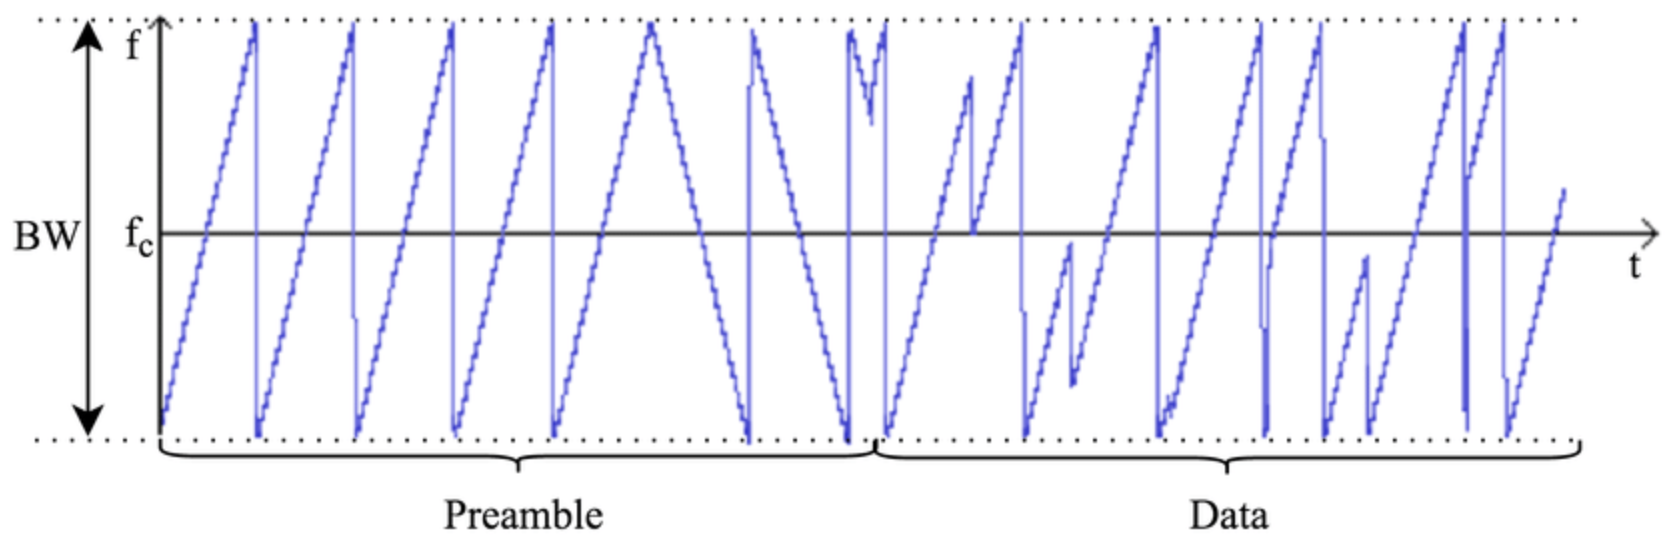
\includegraphics[width=0.9\textwidth]{Figures/StateOfTheArt/lora_modulation_css.png}
    \caption{Modulation \textit{chirp spread spectrum} de LoRa}
    \label{fig-lora_modulation_css}
\end{figure}


Le principe CSS de la modulation LoRa est visible sur la \cref{fig-lora_modulation_css} illustrant une trame LoRa utilisant cette même modulation. Le codage des informations consiste donc en la dérivée de la fréquence en fonction du temps, afin de coder les diverses informations désirées. Les états prennent en compte des valeurs précédentes et incluent des alignements sur les données afin de réduire l'impact du bruit sur le signal. Les tables expliquant le codage de la modulation sont disponibles dans le document de la présentation de Matt Knight au Jailbreak Security Summit.\\


L'un des défauts du LoRa est celui du choix du contrôleur effectuant l'implémentation matérielle de la modulation. À l'heure actuelle, un seul fabricant est autorisé à produire les puces avec la modulation LoRa, il s'agit de la société Semtech. Cela réduit considérablement le nombre de possibilités et détruit également la concurrence dans le domaine, puisque le prix est dicté par le créateur du standard. Semtech a annoncé une collaboration avec STMicroelectronics pour développer un processeur dans lequel on retrouve un STM32, avec en interne, un c\oe ur attribué uniquement à la modulation LoRa et l'implémentation du protocole LoRaWAN. Mais en attendant ce microcontrôleur, Murata, un célèbre fabricant de semiconducteurs, s'est allié avec STMicroelectronics afin d'offrir un module nommé CMWX1ZZABZ-078. Ce module est composé, en interne, d'un STM32L0 et d'un \textit{tranceiver} SX1276 de Semtech. La communication entre ces deux éléments est possible, via l'utilisation d'un bus SPI.

\subsection{Sensibilité}

L'augmentation de la bande passante du signal est le principe fondamental des différentes technologies de communications de type \textit{spread-spectrum}. Sans cela, le transport sur de longues distances ne serait pas possible. La sensibilité de réception du LoRa par rapport à la modulation concurrence FSK est visible sur la \cref{fig-lora_vs_fsk_sensibility} \cite{AN12002292:online}. On constate que le LoRa dispose d'une sensibilité plus importante pour un débit de données égal. Semtech propose une note d'application nommée \texttt{AN1200.22} \footnote{https://www.semtech.com/uploads/documents/an1200.22.pdf} explorant plus en détail la modulation LoRa et ses puissances. Ce même document explique également les différents \textit{noise floor} illustrés en \cref{fig-lora_vs_fsk_sensibility} à l'aide une approche mathématique.

\begin{figure}[ht!]
    \centering
    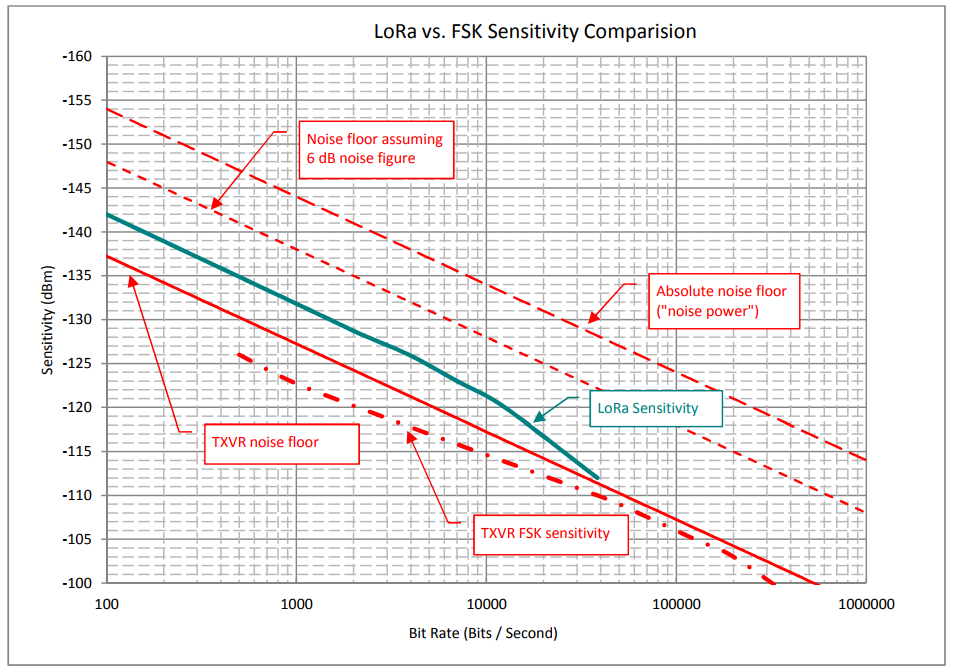
\includegraphics[width=0.9\textwidth]{Figures/StateOfTheArt/lora_vs_fsk_sensibility.png}
    \caption{Comparaison de la sensibilité entre la modulaton FSK et LoRa}
    \label{fig-lora_vs_fsk_sensibility}
\end{figure}


\subsection{\textit{Coding rate}}

En télécommunications, le \textit{coding rate} est utilisé pour ajouter une correction d'erreur lors de la récupération d'un paquet. Si le \textit{code rate} est de \texttt{k}/\texttt{n}, pour chaque \texttt{k} bits d'information utile, l'encodeur génère au total \texttt{n} bits de données \cite{Coderate2:online}. Cela a pour résultat d'ajouter des données dans un paquet. Dans le cas de LoRa, cela augmente temps d'émission, réduisant ainsi le nombre de paquets qui peuvent être envoyés par unité de temps. 

\subsection{\textit{Spreading factor}}
\label{sec-stateoftheart_lora_spread_factor}

Le \textit{Spreading Factor} (SF) est un facteur qui est calculé en tenant compte de la durée d'un décalage en fréquence. Par exemple, sur la \cref{fig-lora_modulation_css} il s'agit du temps que met le \textit{shift} pour parcourir BW. LoRa opère avec des \textit{Spreading Factors} de 7 à 12. Chaque incrémentation de 1 du SF, double le temps d'émission d'un \textit{chirp} \cite{Explorat95:online}. Ce qui a pour conséquence --- avec la même bande passante --- d'augmenter le temps d'émission et donc réduire le débit de données.


\subsection{Structure des paquets}

La spécification LoRa décrit essentiellement l'implémentation d'une modulation. Cependant, une partie de la couche 2 du modèle OSI\footnote{\url{https://en.wikipedia.org/wiki/OSI_model}} est également affectée par cette spécification. 
Ce paquet est constitué des éléments présentés sur la \cref{fig-lora_packet}. 
\begin{figure}[ht!]
    \centering
    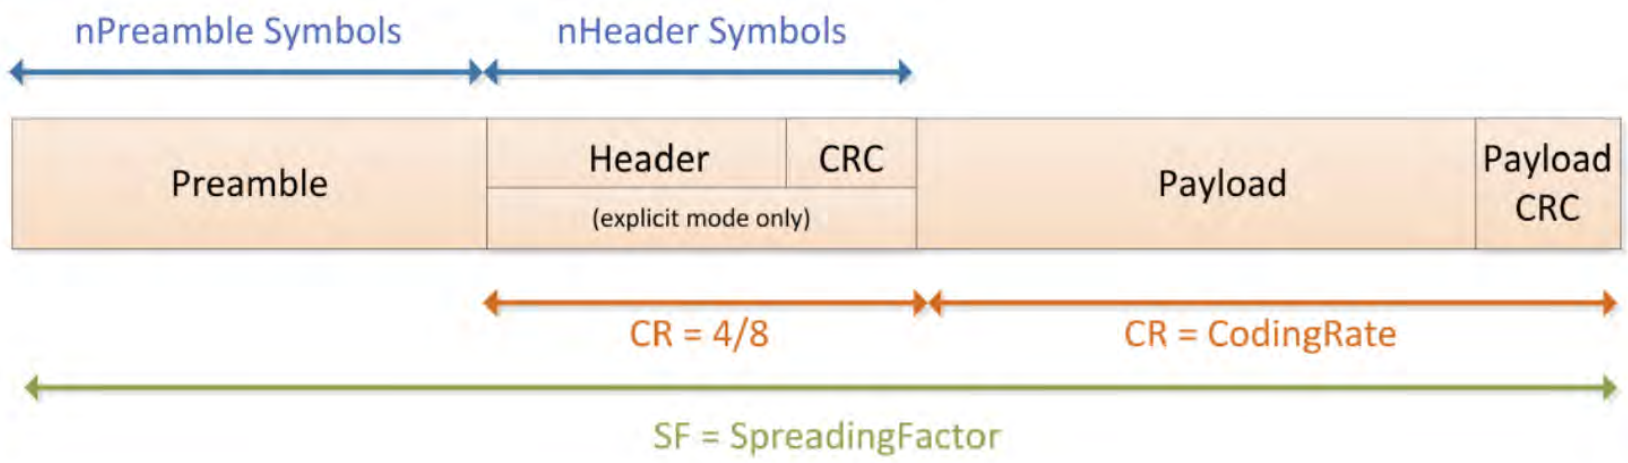
\includegraphics[width=0.9\textwidth]{Figures/StateOfTheArt/lora_packet.png}
    \caption{Composition d'un paquet LoRa}
    \label{fig-lora_packet}
\end{figure}

Un paquet LoRa commence toujours avec un préambule constant qui couvre toute la bande de fréquence contenant à la fin un byte de synchronisation \cite{AStudyof31:online}. Ce byte permet ainsi de différencier les différents réseaux LoRa qui utilisent les mêmes bandes de fréquences. Un périphérique configuré pour écouter un byte de synchronisation précis va s'arrêter si le byte décodé ne correspond pas au byte attendu. La taille du préambule est configurable entre 10.25 et 65539.25 symboles \cite{AStudyof31:online}. Une image du préambule dans le domaine fréquentiel est visible sur la \cref{fig-lora_modulation_css}.\\

Suivant le préambule, il y a un entête qui est optionnel. Si celui-ci est présent, il est toujours envoyée avec un \textit{coding rate} de 4/8. Cet entête a pour but d'indiquer la taille du \textit{payload} en bytes, le \textit{coding rate} utilisé pour le reste de la transmission, ainsi que spécifier si la trame finit par un CRC 16-bit ou non. L'entête inclut son propre CRC pour éviter les erreurs et ainsi ignorer le paquet au cas où il aurait été corrompu. La taille du \textit{payload} est définie uniquement à l'aide d'un \textit{byte}, ce qui limite la taille totale du \textit{payload} à 255 \textit{bytes} \cite{AStudyof31:online}. L'entête n'est pas requis lorsque le \textit{payload} a une taille fixe et que le récepteur connait la configuration du paquet (taille \textit{payload}, \textit{coding rate} et si un CRC est présent ou non).


\FloatBarrier
\subsection{Distance d'émission}
\begin{figure}[ht!]
    \centering
    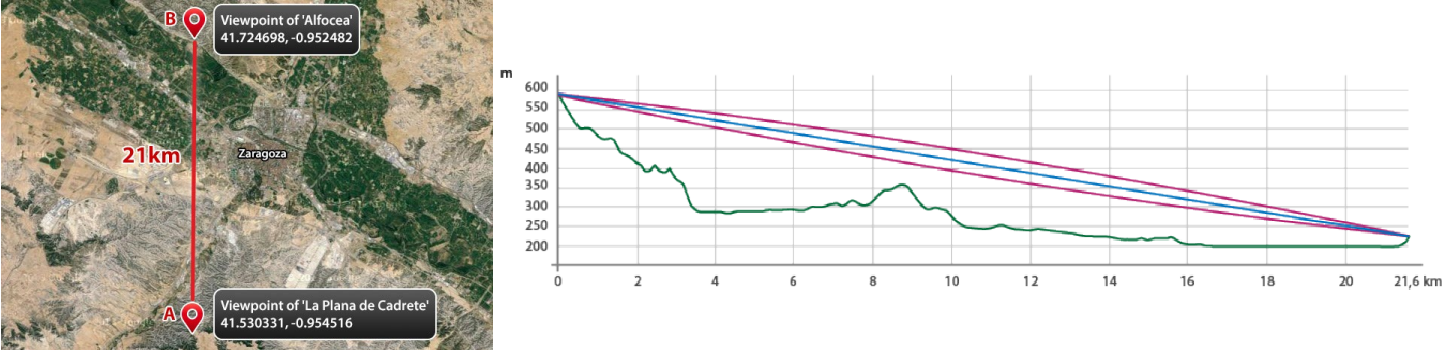
\includegraphics[width=1.0\textwidth]{Figures/StateOfTheArt/lora_distance_measure.png}
    \caption{Tests de portée à l'aide de deux dispositifs LoRa avec visualisation de la topologie du terrain}
    \label{fig-lora_distance_measure}
\end{figure}
L'entreprise Libelium\footnote{\url{http://www.libelium.com/}}, spécialisé dans la production et la vente de plateformes de développement IoT, a effectué plusieurs tests sur la portée du LoRa \cite{waspmote8:online}. Pour ce faire, deux périphériques ont été placés à 21\,km de distance dans une zone non urbaine. Le placement de ces périphériques est visible sur la \cref{fig-lora_distance_measure}, où il est possible de voir à gauche une localisation GPS et à droite le profil du terrain. On constate un dénivelé entre les deux périphériques d'environ 400\,m.\\

Plusieurs mesures ont été effectuées entre les deux périphériques en appliquant différents paramètres. Ces résultats sont visibles en \cref{fig-lora_distance_array}. Les modes définissent une combinaison de \textit{bandwidth} (BW), de \textit{coding rate} et de \textit{spread factor} (SF) décrits en détail à l'aide de la \cref{fig-lora_mode_libelium}. La modification de ces paramètres change la sensibilité d'émission et de réception. En analysant les différents résultats, on constate que le taux de réception des paquets est très élevé, avec des résultats proches de 100\,\% dans trois modes \cite{waspmote8:online}. Le mode 9 se révèle quant à lui inadapté pour ce type de transfert, il est donc à proscrire pour de longues distances.

\begin{figure}[ht!]
    \centering
    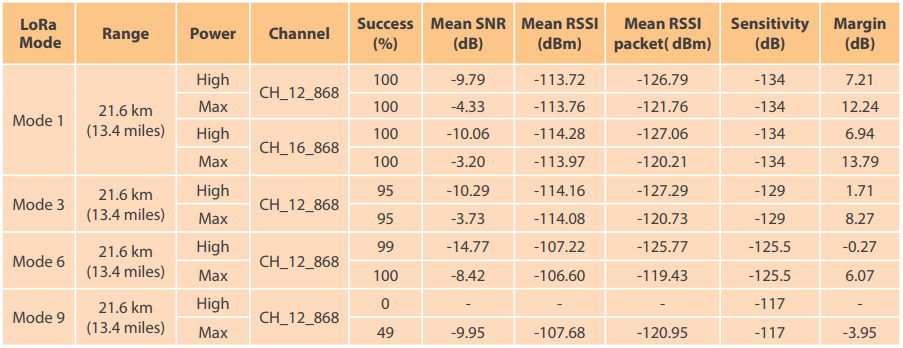
\includegraphics[width=1.0\textwidth]{Figures/StateOfTheArt/lora_distance_array.png}
    \caption{Résultats des distances maximales LoRa réalisées par Libelium}
    \label{fig-lora_distance_array}
\end{figure}

\begin{figure}[ht!]
    \centering
    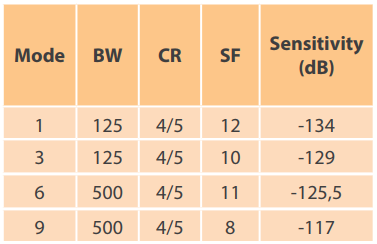
\includegraphics[width=0.32\textwidth]{Figures/StateOfTheArt/lora_mode_libelium.png}
    \caption{Description des modes utilisés par Libelium}
    \label{fig-lora_mode_libelium}
\end{figure}



\FloatBarrier
\subsection{Cycle d'opération}
\label{sec-stateoftheart_lora_dutycycle}

Le cycle d'opération (\textit{duty cycle} en anglais) est grandement limité sur les bandes de fréquences utilisées par le LoRa en Europe. Ces fréquences diffèrent en fonction des pays, mais en Europe les bandes de fréquences autorisées sont 863-870\,MHz et 433\,MHz. Ces cycles d'opérations sont réglementés par la section 7.10.3 du standard ETSI EN300.220 \cite{EN30022033:online} pour l'Europe. Voici le pourcentage de temps que les différentes bandes de fréquences peuvent être utilisés en pourcentage : 
\begin{enumerate}
    \item g (863.0 – 868.0\,MHz): 1\,\%
    \item g1 (868.0 – 868.6\,MHz): 1\,\%
    \item g2 (868.7 – 869.2\,MHz): 0.1\,\%
    \item g3 (869.4 – 869.65\,MHz): 10\,\%
    \item g4 (869.7 – 870.0\,MHz): 1\,\%
\end{enumerate}

On constate qu'il s'agit d'une restriction considérable sur l'envoi des données. Le pourcentage est basé sur le temps total d'une heure. C'est-à-dire que pour le cas des 1\,\%, on ne peut émettre que pendant 36 secondes par heure. Le temps d'émission d'un paquet peut être de plusieurs secondes, selon le type de \textit{coding rate} et \textit{spreading factor} choisi.


La puissance est également spécifiée par ETSI pour les différents canaux possibles dans leur document.


\section{LoRaWAN}

LoRaWAN définit le protocole de communication alors que LoRa est la couche physique sur laquelle se repose le protocole LoRaWAN. LoRaWAN opère principalement en couche 2 du modèle OSI, en tant que \textit{medium access control} (MAC). Les données envoyées au travers d'un réseau LoRa sont chiffrées en AES-128\footnote{\url{https://en.wikipedia.org/wiki/Advanced_Encryption_Standard}}. Le protocole LoRaWAN est exploré plus en \cref{sec-protocols_lorawan} de ce document. La sécurité LoRaWAN est, quant à elle, explorée en \cref{sec-security_lorawan}.\\

LoRaWAN autorise l'envoi de données bidirectionnelles, mais les messages \textit{downlink} (de l'application jusqu'aux périphériques) ne sont transmissibles que sous certaines conditions.

L'implémentation du protocole LoRaWAN est fait uniquement en logiciel. La plupart des implémentations proposées par les fabricants de microcontrôleurs sont basées sur le code de Semtech nommé LoRaMAC-node\footnote{\url{https://github.com/Lora-net/LoRaMac-node}}. Ceci permet ainsi de faciliter ainsi le développement sur les microcontrôleurs qui sont couplés aux contrôleurs LoRa vendus.


\section{Communication sans fil à 2.4 GHz}
\label{sec_2_4_GHz}

La plage de fréquence autour de 2.4\,GHz est l'une des plus utilisée. Ceci est dû au fait que celle-ci peut être exploitée sans nécessiter l'obtention d'une licence provenant d'une autorité de certification et cela dans tous les pays \cite{ISMbandW77:online}. Plusieurs autres fréquences sont également ouvertes dans le monde, mais le succès de cette plage provient de trois facteurs : 
\begin{itemize}
    \item la taille de l'antenne. En effet, un principe simple en radio communication est que plus la fréquence est élevée et plus l'antenne peut être compacte. On peut facilement le constater avec l'\autoref{eq:dipole_base_formula} représentant la longueur d'un dipôle \cite{DipoleLe18:online}. La constante A dépend principalement de la longueur de l'antenne en fonction de l'épaisseur du matériau utilisé. Cette constante se situe typiquement entre 0.96 et 0.98 \cite{DipoleLe18:online}. Il est possible de trouver divers graphiques permettant d'obtenir la valeur de cette constante \footnote{\url{http://www.radio-electronics.com/info/antennas/dipole/length-calculation-formula.php}}, facilitant ainsi son dimensionnement.
    
    
    \begin{equation}
    \label{eq:dipole_base_formula}
    \text{Longueur dipôle }[m] = \frac{150 \times A}{freq [MHz]}
    \end{equation}

    \begin{equation}
    \label{eq:dipole_2_4GHz}
    \text{Longueur dipôle }[m] = \frac{150 \times 0.98}{2400} = 0.06125 = 6.125 [cm]
    \end{equation}
    
    \begin{equation}
    \label{eq:dipole_433MHz}
    \text{Longueur dipôle }[m] = \frac{150 \times 0.98}{433} \approx 0.33949 = 33.949 [cm]
    \end{equation}
    
    En utilisant l'\autoref{eq:dipole_base_formula} avec 2.4\,GHz (\autoref{eq:dipole_2_4GHz}) et 433\,MHz (\autoref{eq:dipole_433MHz}) on observe bien l'influence de la fréquence sur ce dipôle et la place qui devra être allouée à une antenne sur une carte électronique. Grâce à une miniaturisation qui devient raisonnable, on peut facilement offrir des périphériques compacts.\\
    
    \item la technologie électronique disponible pour gérer ces hautes fréquences. Grâce à l'avancée dans les domaines de l'électronique et de la microélectronique, il est maintenant possible d'avoir des circuits intégrés pouvant offrir la modulation à cette fréquence et cela en ayant une taille raisonnable. Par exemple, le microcontrôleur utilisé dans ce projet, le KW41Z de NXP, offre un \textit{package} de 3.9x3.8\,mm ne nécessitant aucun élément électronique externe pour l'amplification de l'antenne. Ceci permet de créer une carte électronique extrêmement compacte. Le prix de ce type de technologie est de plus en plus négligeable lors du développement(cf. \autoref{subsect:microcontroleur} pour un comparatif plus approfondi des microcontrôleurs compatibles Bluetooth avec des indications de prix).\\
    
    \item la distance couverte par cette plage de fréquence. Cette fréquence permet d'avoir une distance tout à fait raisonnable entre deux périphériques qui souhaitent interagir. Le Bluetooth 5.0 peut ainsi atteindre, en théorie, jusqu'à 500\,m dans un environnement ouvert, avec son mode \textit{long range}\cite{Explorin32:online}. Bien entendu, selon le type de réseau que l'on souhaite créer cette distance est peut-être trop faible. Cependant, il est toujours possible d'utiliser des protocoles qui implémentent des principes de \textit{mesh networking} afin de propager les messages à travers un réseau de n\oe uds.\\
\end{itemize}

La fréquence de 2.4\,GHz est utilisée par de nombreux protocoles. On y trouve le Bluetooth, le Wi-Fi, ou une multitude d'autres standards, comme le IEEE 802.15.2. Si on prend l'exemple d'un smartphone ou d'une tablette, les seuls protocoles supportés universellement sur toutes ces plateformes sont le Bluetooth, ainsi que le Wi-Fi. Le problème de ce dernier est l'impact sur la consommation des appareils, mais avec comme avantage d'avoir un grand débit de données possibles. Le Bluetooth est lui plutôt utilisé lors de la communication avec des périphériques proches de l'utilisateur et nécessitant un débit de données moyen, mais offrant en contrepartie une plus grande autonomie. Le Wi-Fi est quant à lui utilisé dans le cadre d'un besoin de communication avec des données externes, provenant par exemple d'Internet.\\

%La modulation LoRa est maintenant également disponible dans cette fréquence grâce au circuit intégré Semtech SX1280\footnote{\url{http://www.semtech.com/wireless-rf/rf-transceivers/sx1280/}}. \\


\section{Bluetooth Low Energy}
\label{sec-stateoftheart_ble}

Le standard Bluetooth existe depuis 1994 et a été inventé par Ericsson \cite{Bluetoot45:online}. Il a été premièrement conçu pour créer une alternative à la connexion filaire RS-232. Le standard est maintenu par le \textit{Bluetooth Special Interest Group}\footnote{\url{https://www.bluetooth.com/}}.\\

Le Bluetooth Low Energy initiliament nommé Wibree, a été pensé par Nokia avec une collaboration entre STMicroelectornics et Logitech \cite{Bluetoot45:online}. La sortie publique a été annoncée en 2006. En 2007, le \textit{Bluetooth Special Interest Group} a pris la décision d'implémenter au sein du protocole Bluetooth les concepts avancés par le Wibree. En 2010, la spécification Bluetooth Low Energy en version 4.0 a été annoncée. Il a fallu attendre fin 2011 pour qu'elle fasse son apparition dans les premiers équipements grand public, comme l'iPhone 4S. Les principales différences entre le Bluetooth et le Bluetooth Low Energy sont illustrées sur la \cref{fig-bluetooth_vs_ble}. Il est possible de voir que la grande différence provient du débit. Avec le Bluetooth Low Energy, on limite le nombre de communications afin d'économiser un maximum d'énergie. Cela ouvre la porte à des dispositifs très basse consommation, qui peuvent communiquer durant plusieurs mois, mais en contrepartie limite le nombre de données transitant sur ce type de communication.

\begin{figure}[ht!]
    \centering
    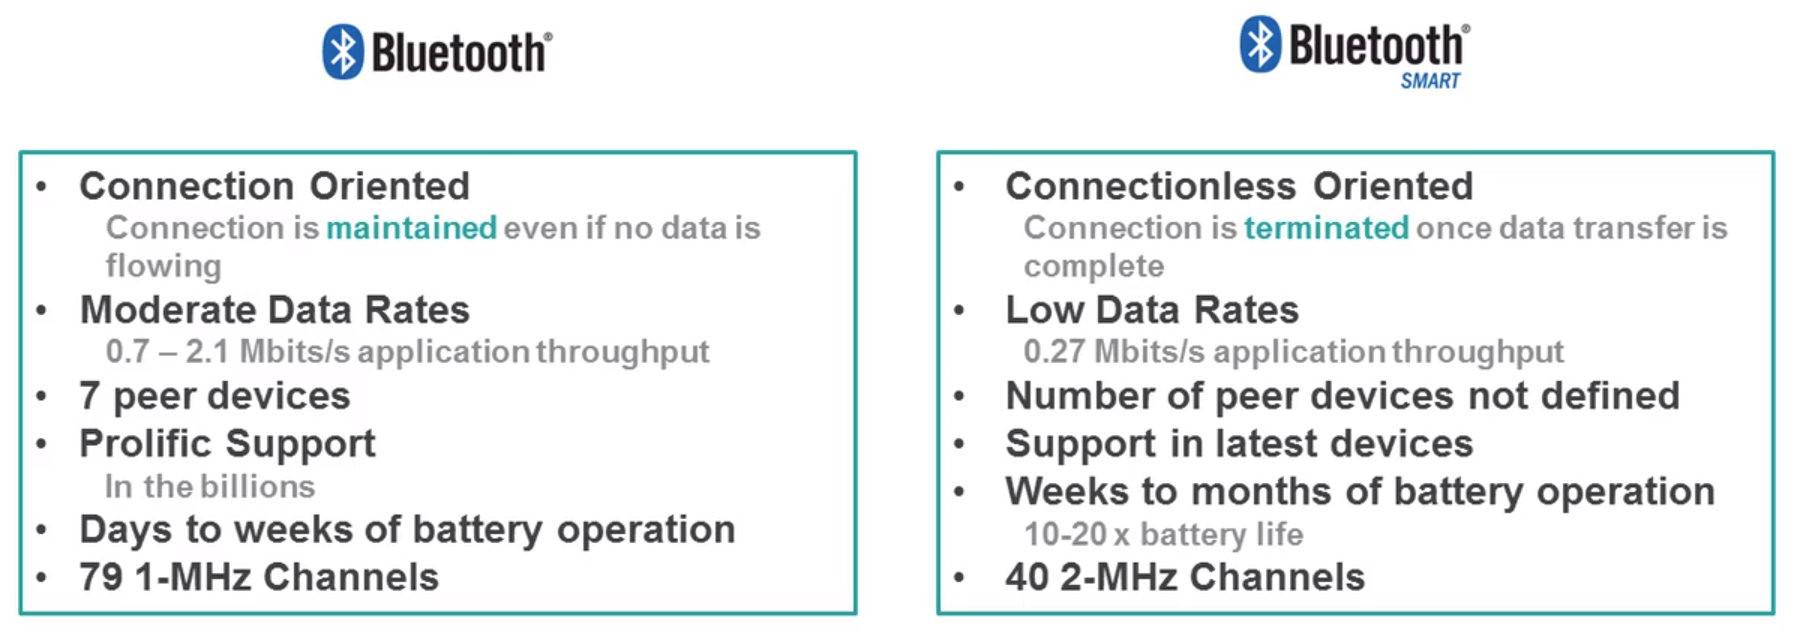
\includegraphics[width=0.9\textwidth]{Figures/Protocols/Bluetooth/bluetooth_vs_ble.PNG}
    \caption{Comparaison Bluetooth et Bluetooth Low Energy}
    \label{fig-bluetooth_vs_ble}
\end{figure}

Le Bluetooth 5.0 a été officiellement annoncé le 16 juin 2016. Néanmoins, les premiers microcontrôleurs implémentant toutes les fonctionnalités de ce protocole n'ont été annoncés que courant 2017. Une partie des prérequis pour passer au Bluetooth 5.0 ne nécessitent qu'une mise à jour logicielle. Par exemple, l'augmentation de la taille des \textit{advertissements}, qui passent de maximum 31 bytes à 255 bytes. Le Bluetooth 5.0 crée également deux nouveaux modes, le mode \textit{long range} (nommé LE Coded) et le mode \textit{high speed} (nommé LE2M)\cite{Explorin32:online}. Le premier offre une distance accrue au détriment du débit, alors que le deuxième mode est son opposé.\\

Le marché du Bluetooth est en pleine expansion depuis plusieurs années. Cette tendance est due à la démocratisation des smartphones. Le Bluetooth est en effet l'une des rares interfaces de communication présente sur ces dispositifs avec les communications cellulaires et WiFi.\\


Le protocole Bluetooth est exploré plus en \cref{sec-protocols_ble}. La sécurité du Bluetooth est quant à elle explorée en \cref{sec-security_ble} de ce document.


\section{IEEE802.15.4}

L'IEEE 802.15.4 est un protocole utilisé dans les communications sans fil et définit par l'association professionnelle \textit{Institute of Electrical and Electronics Engineers} (IEEE)\cite{IEEE802137:online}. Les protocoles utilisant ce standard comme base font partie d'une catégorie nommée \textit{Low Rate Wireless Personal Area Network} (LR WPAN) due à la basse consommation, au faible débit, ainsi que la faible portée de communication. Ce protocole définit trois fréquences d'utilisation possibles : 

\begin{enumerate}
    \item 2.4 à 2,4835\,GHz avec l'utilisation de 16 canaux;
    \item 902 à 928\,GHz avec l'utilisation de 10 canaux;
    \item 868 à 868,6\,GHz avec l'utilisation de 1 canal.
\end{enumerate}


Ces types de protocoles sont principalement présents dans la domotique par le fait de leur basse consommation, mais surtout de l'avantage des réseaux maillés (\textit{mesh networking}). \\

Il est important de faire un petit comparatif des différents protocoles disponibles afin de les comparer au Bluetooth. En effet, plusieurs microcontrôleurs implémentant du Bluetooth peuvent, en parallèle, être membre d'un réseau IEEE802.15.4 (cf. KW41Z de NXP).

\subsection{ZigBee}


Le ZigBee\footnote{\url{http://www.zigbee.org/}} est un protocole très puissant en raison de sa conception, car ce protocole a été pensé pour interconnecter plusieurs périphériques avec la possibilité d'intégrer directement le principe de réseau maillé (\textit{mesh}). Plusieurs architectures sont possibles avec ce réseau, illustrées par la \cref{fig-zig_bee_architecture}. Il a été conçu en 1998 et standardisé en 2003\cite{ZigBeeW24:online}, ce qui fait de lui un protocole reconnu et présent dans beaucoup de réseaux liés à l'IoT.


\begin{figure}[ht!]
\centering
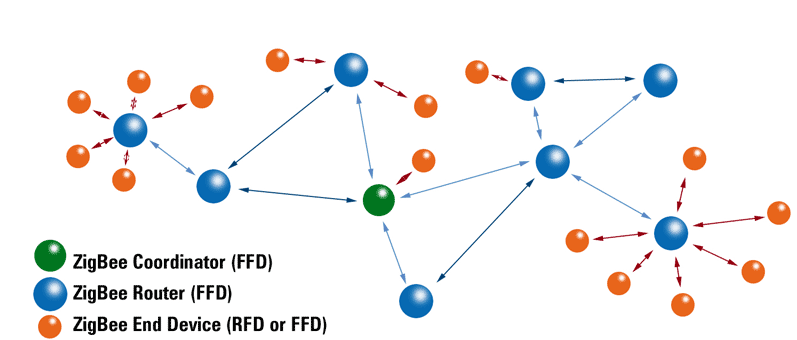
\includegraphics[width=0.9\textwidth]{Figures/StateOfTheArt/zig_bee_architecture.jpg}
\caption{Exemples d'architectures avec la technologie ZigBee}
\label{fig-zig_bee_architecture}
\end{figure}

Un exemple de réseau ZigBee est visible sur la \cref{fig-zig_bee_architecture}. Ces réseaux sont composés de 3 éléments : 
\begin{enumerate}
    \item \texttt{Périphériques} (\textit{End Device}) : sont les éléments qui fournissent les données au réseau, c'est sur ces derniers que les capteurs acquérant les données sont présents. Ce sont ces dispositifs qui sont les moins gourmands en énergie sur le réseau, car ils peuvent dormir la plus grande partie du temps, puis se réveillent pour acquérir les données et/ou les envoyer sur le réseau. Le périphérique doit informer le réseau quand il a été déplacé, mais également interroger son parent pour savoir s'il a reçu un nouveau message.
    \item \texttt{Routeurs} : sont les éléments responsables pour router le trafic entre les différents n\oe uds. Dans certaines implémentations du protocole (version 3.0) \cite{httpswww49:online}, ces routeurs ne peuvent pas dormir. Ce sont donc des éléments qui ne sont pas adéquats pour être alimentés uniquement par batterie.
    \item \texttt{Coordinateur} : est un routeur avec des caractéristiques spéciales\cite{httpswww49:online}. En plus de toutes les tâches du routeur, il a pour rôle de former la topologie du réseau. Pour cela, il doit sélectionner les canaux de communication, les identifiants des éléments du réseau, ainsi que l'adresse du réseau elle-même. Il a également un rôle principal dans la sécurité, car il valide les nouveaux périphériques et contrôle que les données fournies sont de confiance. Les clés de tous les dispositifs du réseau sont également générées par ce dernier.
\end{enumerate}



Le ZigBee est disponible sur les 3 bandes de fréquences autorisées par le standard 802.15.4. Mais certaines de ces fréquences sont limitées géographiquement. La fréquence la plus utilisée est le 2.4\,GHz, du fait de son autorisation internationale. \\


Le routage des paquets ZigBee se produit à deux niveaux\cite{ZigBeeW24:online}. Le premier est au niveau de la couche réseau et peut être de type direct ou indirect. Le routage indirect se produit lorsque le dispositif ne connait pas l'adresse du destinataire. Un n\oe ud de type routeur ou coordinateur fait alors la relation avec le destinataire final en utilisant sa table de routage et sa table de découvertes des routes. Le routage est direct, lorsque le dispositif qui transmet les données connait l'adresse réseau du destinataire.  \\

L'autre type de routage se produit au niveau de l'applicatif en utilisant la table de liaisons stockée dans un coordinateur ou routeur. Les liaisons sont des liens logiques entre des dispositifs d'application complémentaire et des capteurs/périphériques. Le routage au niveau de l'applicatif se fait grâce à la table de liaison, contenu dans le coordinateur ou un routeur. \\

\subsection{Thread}
\label{sec-thread_protocol}

Thread est un protocole basé sur le principe \textit{IPv6 over Low-Power Wireless Personal Area Networks} (6LowPAN)\cite{6LoWPANW35:online}. Les objets d'un réseau Thread sont directement accessibles via des adresses IPV6. Le protocole a été créé par Nest Labs (racheté en 2013 par Google/Alphabet)\cite{Threadne85:online} et est compatible avec tous les produits de la marque Nest. Une des forces de Thread réside dans les partenaires du projet, car on y trouve ainsi tous les grands fabricants de microcontrôleurs comme NXP, Silicon Labs et Texas Instruments, mais également ARM à l'aide des bibliothèques pour mbed OS\footnote{\url{https://www.mbed.com/en/platform/mbed-os/}}. \\

\begin{figure}[ht!]
    \centering
    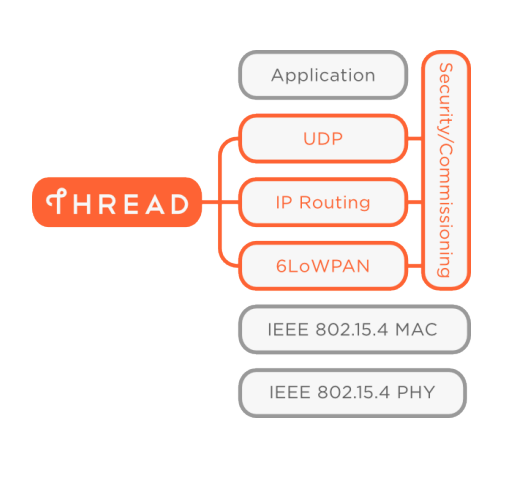
\includegraphics[width=0.6\textwidth]{Figures/StateOfTheArt/thread_stack.png}
    \caption{Architecture d'une \textit{stack} logicielle Thread}
    \label{fig-thread_stack}
\end{figure}

Les différentes couches ajoutées par Thread sont visibles sur la \cref{fig-thread_stack}. On constate que Thread utilise UDP et non TCP pour l'échange de messages. Réduisant ainsi l'\textit{overhead} rajoutée par les paquets UDP et ainsi réduire la complexité pour former les trames de données sur les différents périphériques du réseau. \\

Thread a été construit avec la sécurité comme élément primordial. En effet, tous les messages sont chiffrés en AES-128. La génération des clés et leur échange sont basés sur ECC et J-PAKE\cite{Sevenkey87:online}. Pour ajouter un nouveau capteur au réseau, un périphérique de mise en service connu et approuvé au réseau est nécessaire (ex.: un smartphone). Pour rajouter un capteur, le périphérique de mise en service doit donner l'identifiant du capteur et fournit un mot de passe au réseau. L'échange de ces informations est effectué à l'aide d'une connexion sécurisée basée sur le protocole \textit{Datagram Transport Layer Security} (DTLS), après l'authentification de l'utilisateur.


\begin{figure}[ht!]
    \centering
    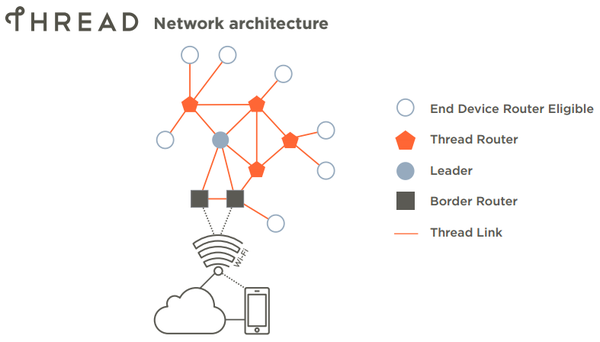
\includegraphics[width=0.9\textwidth]{Figures/StateOfTheArt/thread_architecture.png}
    \caption{Architecture d'un réseau Thread}
    \label{fig-thread_architecture}
\end{figure}

Contrairement au protocole ZigBee, Thread est beaucoup plus dynamique dans son réseau. Cela s'explique par le fait que seulement deux types de n\oe uds sont réellement possibles dans un réseau Thread \cite{Sevenkey87:online}. Un troisième type est ensuite élu par ce même réseau. Voici la définition des types qui sont également visibles sur la \cref{fig-thread_architecture} : 

\begin{enumerate}
    \item \texttt{End Device} : est le capteur qui va fournir des données vers le réseau. Ceux-ci sont souvent alimenté par batterie et ne doivent s'activer que sporadiquement pour être efficients. 
    \item \texttt{Router Eligible} : s'agit d'un \texttt{End Device}, mais pas obligatoirement. Si par exemple, le réseau a besoin d'un nouveau routeur, par grand trafic de données ou lorsque les routes créées ne sont pas assez nombreuses, il devient un routeur sur le réseau. Son but est alors d'écouter l'arrivée de nouveaux paquets et de les rediriger vers le \textit{End Device} de destination ou le routeur le plus proche. Étant donné qu'un routeur doit écouter toutes les communications, il ne pas être considéré comme un périphérique \textit{low power}.
    \item \texttt{Leader} : est un \texttt{Router Eligible} qui se fait élire à ce poste par le réseau. Ce leadeur peut changer au fil du temps, mais un seul peut être actif par réseau. Il doit s'occuper de tâches supplémentaires sur le réseau et de prendre la plupart des décisions.
\end{enumerate}


Les\textit{ border router} sont des routeurs qui proposent un pont vers un autre réseau. Dans l'exemple exposé en \cref{fig-thread_architecture}, un pont Internet ou un réseau local est présent pour que les capteurs soient directement accessibles depuis un smartphone ou un service quelconque. Ces \textit{border routers} peuvent aussi convertir vers d'autres types de technologies, par exemple, vers un réseau Bluetooth.


Les principes de Thread sont similaires à ZigBee, mais l'apport de la technologie IPv6 est un avantage dans l'IoT, car cela facilite l'accès aux capteurs depuis un réseau externe.


%-----------------------------------------------------------------------------------
\section{Équipements matériels existants}
%-----------------------------------------------------------------------------------




Il existe sur le marché divers fabricants proposant des kits de développement orientés IoT et très facilement utilisables dans un concept \textit{SmartCity}. L'un des plus connus est STMicroelectronics\footnote{\url{http://www.st.com/content/st_com/en.html}}, car il propose une très grande panoplie de capteurs pouvant êtres utilisés dans un grand nombre de situations\footnote{\url{http://www.st.com/en/evaluation-tools/stm32-nucleo-expansion-boards.html}}. Les kits de développement de STM sont souvent utilisés par des passionnés, au vue de leur de disponibilité et de leur faible cout sur le marché. Des kits avec du WiFi, du NFC et du Bluetooth peuvent être achetés pour moins de 50\,CHF. L'écosystème STM dispose d'une très grande communauté, ainsi que de bibliothèques très bien construites qui facilitent l'implémentation d'un projet personnel. Une grande partie de leurs kits de développement sont supportés par la plateforme mbed\footnote{\url{https://www.mbed.com/en/}}, maintenue par la société de conception d'architecture de processeurs ARM. La plateforme mbed offre ainsi une suite de bibliothèques facilitant l'implémentation et la programmation. Un problème provenant de ces kits est la disponibilité. Ces kits ne sont pas censés être utilisés pour des produits définitifs. Ils sont uniquement des plateformes de tests pour le produit vendu, ce qui n'oblige aucunement le vendeur à garantir une disponibilité ni même une compatibilité entre les futurs designs. La production de ces kits peut ainsi être interrompue du jour au lendemain. Générant une situation inacceptable si cette carte est utilisée dans un produit commercial. Ils ont comme objectif de réaliser très facilement des prototypes permettant ainsi de créer des \textit{proof of concept} rapidement. Toutefois, lorsque l'utilisateur désire avoir un produit final, il est forcé d'implémenter le processeur directement dans une carte électronique sur mesure. Plusieurs acteurs proposent des kits sur le marché. Les plus grands fabricants de microcontrôleurs sont STM, NXP ou Texas Instruments, proposant chacun des plateformes et des exemples afin de tester leurs produits. \\

Les dispositifs matériels sur le marché implémentant une interface de communication utilisent parfois deux processeurs. Un premier processeur, souvent le moins puissant, est utilisé pour la gestion de l'interface de communication. Il s'occupe à lui seul de la communication avec l'extérieur. Ceci peut s'avérer une tâche couteuse selon le type de protocole implémenté. Par exemple, lorsque de la cryptographie est utilisée, le chiffrement et déchiffrement des paquets peut être couteux en temps de calcul. Ce processeur communique ensuite avec un processeur plus puissant via une interface de communication variant selon les implémentations. Un deuxième processeur est à disposition de l'utilisateur pour toutes les tâches qu'il souhaite effectuer. Mais il ne faut pas oublier que la communication avec le premier processeur aura un impact sur les performances. À cause de ce type de structure, mais aussi de la complexité à maintenir un système stable, un \textit{Real-Time Operating System} (RTOS) est souvent utilisé.\\

Libelium\footnote{\url{http://www.libelium.com/}} est également un acteur dans le marché des \textit{Smart Cities}. La différence avec STMicroelectronics réside dans le fait que Libelium n'est pas un fabricant de microcontrôleurs en tant que tel. Cette entreprise propose plusieurs cartes dont la plupart sont basées sur un processeur d'Atmel, un ATMEGA1281. Cela permet une utilisation aisée de leurs équipements, mais limite malheureusement la puissance de calcul. Ces processeurs ne sont pas très puissants et l'utilisation de l'environnement Arduino pour la programmation réduit considérablement la flexibilité et la puissance de calcul pour l'utilisateur. Un autre défaut des plateformes Arduino est l'absence d'une interface de débogage (ex. JTAG\footnote{\url{https://en.wikipedia.org/wiki/JTAG}}).\\

Dans l'industrie électronique, un périphérique produit à grande échelle sera toujours réalisé avec la plus grande maitrise possible sur l'implémentation, qu'elle soit matérielle ou logicielle. Un travail de Master doit refléter un besoin de l'industrie et valoriser de nouvelles compétences pour l'étudiant. Toutes ces raisons ont incité la réalisation d'une carte de développement personnalisée pour ce projet. 



% Les \textit{Smart Cities} ne sont rien sans les capteurs qui peuvent fournir les données au réseau, c'est pourquoi, plusieurs entreprises proposent des capteurs qui s'intègrent rapidement sur un réseau existant. Dans le cadre de ce projet, il n'est pas désiré d'avoir un capteur qui fait uniquement un seul type d'acquisitions. L'idéal est d'avoir une carte sur mesure, afin de faciliter les tests de plusieurs scénarios, sans avoir besoin d'apprendre à maitriser un nouvel écosystème à chaque nouveau test.\\


\section{Développement de logiciels sur microcontrôleur}

Cette section a pour but d'explorer l'état actuel des systèmes d'exploitation et des diverses bibliothèques utilisables sur des systèmes embarqués. Dans le cadre de ce projet, deux microcontrôleurs ont été utilisés, l'aspect logiciel a donc été exploré pour connaitre les différentes approches possibles.


\subsection{Stacks Bluetooth}

Le problème lorsque l'on utilise un microcontrôleur avec une interface Bluetooth ou de manière générale un quelconque protocole radio réside dans le fait que le code source s'occupant de la partie radio n'est que très rarement \emph{open source}. Il est souvent distribué sous forme binaire avec une documentation principalement applicative, sans aucune documentation du fonctionnement interne du code (via des machines d'états, etc.). Ce code est souvent référé en tant que \textit{stack RF}.\\

On trouve tout de même certaines \textit{stacks RF} tierces, comme la \textit{stack} BTstack\footnote{\url{https://github.com/bluekitchen/btstack}} développée par l'entreprise Bluekitchen \footnote{\url{http://bluekitchen-gmbh.com/}} et la communauté \textit{open source}. Toutefois le nombre de microcontrôleurs supporté se limite souvent à des microcontrôleurs assez anciens ou simplement ceux très appréciés par le milieu des amateurs de circuits électroniques ou de systèmes embarqués. On trouve ainsi le support des ESP32 du fabricant Espressif Systems, un des microcontrôleurs le plus prisé des hobbyistes par son très faible cout (moins de 4  dollars pour une seule unité sur des sites de ventes comme AliExpress). On a également ceux basés sur les MSP430 de Texas Instruments. Un microcontrôleur assez ancien (sorti en 2010), mais qui est encore l'un des plus connus de Texas Instruments par sa très basse consommation et sa simplicité.

\subsection{Stacks LoRaWAN}

La \textit{stack} LoRaWAN est principalement développé par Semtech à l'aide du projet LoRaMac-node\footnote{\url{https://github.com/Lora-net/LoRaMac-node}}. Cette \textit{stack} requière uniquement au développeur de fournir des fonctions d'écriture et de lecture sur le bus série connecté au périphérique LoRa. La gestion des interruptions doit aussi être mise en place. Le protocole LoRaWAN est géré en intégralité par une machine. Son implémentation est entièrement séquentielle, la présence d'un RTOS n'est donc pas nécessaire.

\subsection{RTOS}
\label{sec-stateoftheart_rtos}

Pour l'implémentation logicielle, plusieurs alternatives sont possibles. Dans le cas de l'utilisation de processeurs implémentant des communications sans fil, un \textbf{Real Time Operating System} (\textit{RTOS}) est très souvent nécessaire et conseillé. Cela est dû au fait que la partie radio est gérée par une tâche propre, souvent doté d'un niveau de priorité supérieur aux autres tâches, afin d'avoir la meilleure réactivité sur les différentes opérations.\\


La différence entre un système en \textit{bare-metal} et un RTOS est visible sur la \cref{fig-rtos_vs_baremetal} \cite{GeneralR94:online}. Un code complexe en \textit{bare-metal} utilise une machine d'état dans une boucle infinie. Cette machine scrute des fanions modifiés par des événements (ex. une ISR\footnote{\url{https://en.wikipedia.org/wiki/Interrupt_handler}}). Dans un RTOS, plusieurs tâches attendent en parallèles sur des événements générés par le déblocage de verrous (sémaphores ou mutexes). Le noyau principal d'un RTOS est l'ordonnanceur (\textit{scheduler}), qui gère l'ordre d'exécution des tâches en fonction des priorités assignées à celles-ci.
\begin{figure}[ht!]
    \centering
    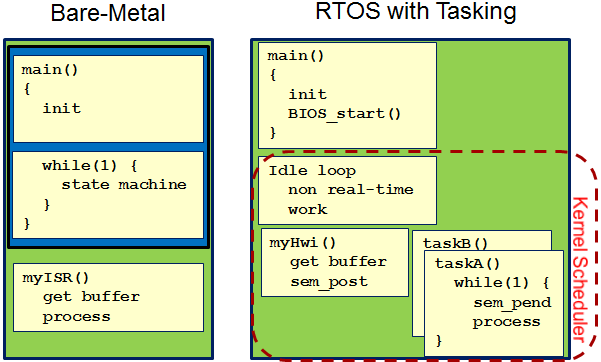
\includegraphics[width=0.9\textwidth]{Figures/StateOfTheArt/rtos_vs_baremetal.png}
    \caption{Comparaison entre RTOS et bare metal}
    \label{fig-rtos_vs_baremetal}
\end{figure}



Il est toujours possible de programmer en \textit{bare-metal}, mais ce type de programmation devient de plus en plus difficile, suite à la complexification grandissante des systèmes connectés. Toutefois, un RTOS crée une surcouche trop importante pour garantir certaines contraintes. Cela arrive souvent avec des contraintes temporelles, quand une application nécessite de faire des opérations avec une grande réactivité \cite{Baremeta22:online}. Mais dans le cas de communication sans fil, une approche \textit{bare-metal} est souvent trop complexe pour être possible. Une autre solution est l'utilisation de deux processeurs, un premier qui gère la communication sans fil, le deuxième s'occupe du reste des opérations. Le processeur RF est donc considéré comme un coprocesseur dans cette architecture. La communication entre ces deux processeurs dépend ensuite des choix du fabricant et non du développeur. 


\subsubsection{FreeRTOS}
\label{sec-RTOS_freertos}

Sur le marché on retrouve divers systèmes d'exploitation. L'un des plus connus est FreeRTOS, parce qu'il est intégralement \textit{open source}\footnote{\url{https://sourceforge.net/projects/freertos/}}. Son succès a été porté sur plus d'une cinquantaine d'architectures \cite{FreeRTOS23:online}. \\

Les dispositifs IoT sont de plus en plus complexes et connectés. L'une des raisons qui ont poussé l'un des leadeurs des produits \textit{cloud} dans ce domaine, Amazon IoT, a développer avec l'organisation FreeRTOS un RTOS modifié\footnote{\url{https://aws.amazon.com/freertos/}} afin de s'intégrer au mieux avec leurs plateformes. Par défaut, les constructeurs de microcontrôleurs fournissent une variante d'un RTOS. Très souvent, cette variante est FreeRTOS, car elle peut être distribuée sans avoir de couts liés aux licences car étant basée sur une licence MIT. \\

\begin{figure}[ht!]
    \centering
    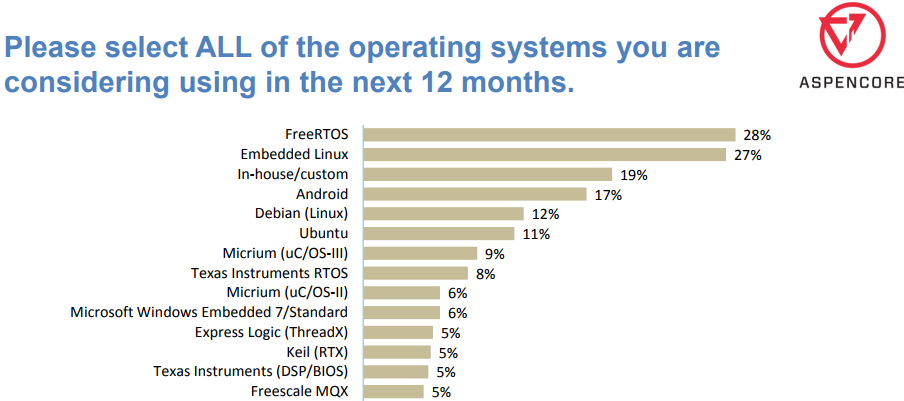
\includegraphics[width=1.0\textwidth]{Figures/StateOfTheArt/embedded_markets_study_2017.PNG}
    \caption{Résultats d'une étude de marché sur les OS réalisée par EE Times et embedded.com en avril 2017}
    \label{fig:eetimes_2017_market_study}
\end{figure}

En avril 2017, le magazine EE Times en collaboration avec le site Internet Embedded.com, tous les deux spécialisés dans les informations sur le monde des systèmes embarqués, ont à nouveau publiés une étude sur la part de marché des systèmes d'exploitation utilisés sur les divers systèmes embarqués\cite{2017Embe35:online}. Cette étude a été réalisée en questionnant les diverses personnes inscrites sur ces deux sites. Au total, 1'234 utilisateurs ont été retenus pour l'année 2017, avec un niveau de confidence de 95\,\% $\pm$ 2.8\,\%. Plusieurs questions ont été posées dans ce sondage, dont celle de nommer tous les OS sur lesquels ils risquent de travailler dans les douze prochains mois. La \autoref{fig:eetimes_2017_market_study} illustre les résultats de cette question. On constate que le premier OS est FreeRTOS, cité par 28\,\% des personnes. 
Néanmoins, cette étude ne se concentre pas sur les systèmes embarqués uniquement réservés à une approche sans fil, basse consommation et avec une faible empreinte, comme dans le cadre de ce travail de Master. Certains de ces OS sont également bien trop complexes pour être utilisables sur des petits microcontrôleurs, c'est pour cela qu'on peut y voir des systèmes d'exploitation très complets comme Ubuntu. Les autres OS utilisables par des microcontrôleurs listés par cette étude et toujours visibles sur la \autoref{fig:eetimes_2017_market_study} sont ceux du développeur Micrium\footnote{\url{https://www.micrium.com/rtos/}}. Il s'agit de deux RTOS nommés µC/OS-III et µC/OS-II. Ce sont par contre deux solutions propriétaires qui nécessitent le paiement de licences pour être utilisées. Cette dernière raison est probablement celle qui fait que FreeRTOS est aussi populaire dans le monde professionnel.


\FloatBarrier
\subsubsection{Zephyr}

\begin{figure}[ht!]
    \centering
    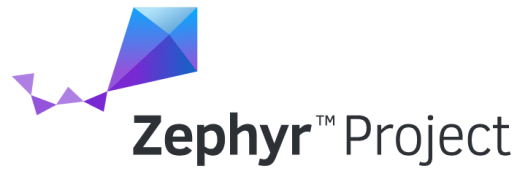
\includegraphics[width=0.55\textwidth]{Figures/StateOfTheArt/zephyr_logo.png}
    \caption{Logo \textit{Zephyr Project}}
    \label{fig:zephyr_logo}
\end{figure}

Le projet Zephyr, lancé le 17 février 2016 \cite{Zephyrop38:online}, est un système d'exploitation temps réel supportant un large éventail d'architectures. Ce projet est porté par la fondation Linux et a pour principal objectif de forcer la sécurité dans les systèmes embarqués avec des implémentations simples, mais efficaces \cite{Zephyrop38:online}. Grâce au support de la fondation Linux, ce projet est extrêmement actif. Une nouvelle version est en moyenne disponible tous les 1 à 2 mois. La documentation est très complète avec plusieurs exemples afin de faciliter l'intégration aux développeurs.

Zephyr a plusieurs caractéristiques qui le différencie de certains concurrents, ce qui le rend attractif dans certains domaines : 
\begin{enumerate}
    \item \textit{Single address-space} : l'application et le kernel utilisent la même plage d'adresse. Ces deux entités, une fois combinées créent une image monolithique qui sera ensuite exécutée sur le système embarqué.
    
    \item Hautement configurable : le \textit{kernel} et l'application peuvent être configurés à l'aide d'une interface afin d'activer uniquement les éléments qui sont nécessaires. Cette interface se base sur le même principe que le noyau Linux à l'aide d'un \textit{Makefile menuconfig}\footnote{\url{https://en.wikipedia.org/wiki/Menuconfig}}.
    
    \item \textit{Compile-time resource definition} : toutes les ressources sont définies à la compilation, ce qui réduit la taille du code source et augmente les performances des systèmes.
    
    \item Vérification minimale des erreurs : afin d'augmenter les performances lors de l'exécution ainsi que la taille du code, il est possible de désactiver la vérification d'erreurs lors de la compilation de l'image. Une option est toutefois disponible pour ne pas les désactiver et ainsi faciliter le débogage des applications lors du développement. 
    
    \item Une suite de services pouvant être complétée au gré de l'utilisateur est disponible. Voici une liste exemplative de services sont déjà implémentés : 
        \begin{itemize}
            \item Un service de \textit{multi-threading} avec la possibilité d'être préemptif avec un ordonnanceur en \textit{round robin}.
            \item Un service de gestion d'interruption qui gère toute la gestion de celles-ci, ainsi que leur enregistrement.
            \item Un service de gestion de l'allocation et de désallocation de la mémoire dynamique (la taille de la mémoire allouée à ce service doit être prédéfinie en avance).
            \item Service de synchronisation \textit{inter-threads} avec l'implémentation de sémaphores, sémaphores compteurs et de mutexes.
            \item Service d'envoi et de réception de données entre les \textit{threads} à l'aide de queues de message et \textit{bytes streams}.
            \item Service de gestion de l'alimentation avec la possibilité de se mettre en mode \textit{idle}, ainsi que d'autres modes basse consommation compatibles avec le matériel utilisé.
        \end{itemize} 
    
\end{enumerate}

Zephyr supporte de multiples architectures telles que ARM Cortex-M, Intel x86, ARC, NIOS II, Tensilica Xtensa et RISC-V. Certaines cartes de développement sont supportées, telles que les ST Nucleo ou les nRF51 de Nordic Semiconductor. Toutefois, le grand défaut de ce framework réside dans le fait que les interfaces radio des différents microcontrôleurs ne sont pas supportées. Par exemple, seuls les microcontrôleurs Bluetooth nRF51 et nRF52 sont supportés. Trois cartes de développements de NXP sont prises en charge (NXP FRDM-K64F, NXP FRDM-KL25Z et NXP FRDM-KW41Z), toutes équipées de Bluetooth Low Energy, mais pas supportées par Zephyr. 

\FloatBarrier
\subsubsection{Mynewt}

\begin{figure}[ht!]
    \centering
    
\includegraphics[width=0.35\textwidth]{Figures/StateOfTheArt/mynewt_logo.png}
    \caption{Logo \textit{Apache Mynewt}}
    \label{fig:mynewt_logo}
\end{figure}

Le RTOS Apache Mynewt est entièrement \textit{open source} et a la même philosophie que Zephyr, c'est-à-dire, la sécurité avant tout . Il est développé avec le support de la très connue \textit{Apache Software Foundation}. Son optique est le monde IoT avec des périphériques connectés, que ce soit via une technologie sans fils ou filaire. Voici les principales caractéristiques de cet OS :

\begin{itemize}
    \item Support BLE 5.0 avec une stack Bluetooth personnalisée;
    \item Support LoRa PHY et LoRaWAN avec le \textit{transceiver} SX1276;
    \item Support du Bluetooth Mesh\footnote{\url{https://blog.bluetooth.com/introducing-bluetooth-mesh-networking}};
    \item Support pour TCP/IP et UDP;
    \item Support pour des \textit{Constrained-Node Networks\footnote{\url{https://tools.ietf.org/html/rfc7228}}} (ex: CoAP, 6LoWPAN).
\end{itemize}


Sa première \textit{release} officielle a été le 24 février 2016\footnote{\url{https://github.com/apache/mynewt-core/releases?after=mynewt_0_9_0_rc1_tag}}. Un RTOS qui est très jeune, tout comme Zephyr, mais qui reste toutefois très intéressant et dont le développement autour de celui-ci semble prometteur. Une \textit{release} majeure est déployée tous les trois mois, ce qui montre une forte implication de la part de la communauté dans le développement de ce projet.

La principale problématique de l'utilisation de ce RTOS est la même que Zephyr, à savoir, le nombre de périphériques actuellement supportés. Pour les périphériques Bluetooth, ce sont principalement les microcontrôleurs de Nordic Semiconductor qui sont supportés en intégralité. Il s'agit de la gamme de modèles NRF51 et NRF52. Dans la liste des microcontrôleurs on retrouve également plusieurs \textit{chip} du fabricant NXP, comme le K64F ou le KW41Z. Ce premier a une interface Bluetooth et Ethernet. Cependant, à l'heure actuelle, uniquement l'interface Ethernet semble être supportée par Mynewt, ce qui n'as pas forcément de sens lorsque l'on souhaite utiliser un microcontrôleur offrant une interface Bluetooth. \\

Pour le LoRa, on peut utiliser n'importe quel type de microcontrôleur compatible avec Mynewt et ensuite connecter un SX1276 via une interface SPI. Mynewt propose ensuite tout un écosystème pour communiquer avec ce périphérique en lui assignant une tâche propre.
Par défaut, les exemples de codes utilisant LoRaWAN reposent sur deux modules, le EE-02 et EE-04\footnote{\url{https://www.telenor.com/innovation/telenor-digital/}}. Ces modules ont été développés par l'entreprise Telenor Digital et les schémas de ces modules sont disponibles sous licence Open Hardware du CERN\footnote{\url{https://github.com/telenordigital/ee0x-hardware}}. Ce module est équipé d'un nRF52832 du fabricant ainsi que du module SX1276 de Semtech. Malheureusement, aucun fournisseur ne semble proposer ce module directement à la vente à l'heure actuelle. 

\subsubsection{Couches d'abstraction}
\label{sec-rtos_abstract_layer}

Certains constructeurs de microcontrôleurs supportent plusieurs RTOS et essayent de faciliter le changement de RTOS à ses utilisateurs. Freescale a donc créé un \textit{framework} nommé Connectivity Framework. Celui-ci, uniquement compatible avec ses microcontrôleurs, a pour but de simplifier le changement de RTOS, d'uniformiser les diverses API et donc d'accélérer le processus de développement. \\

Les microcontrôleurs développés par Freescale (racheté par NXP) sont compatibles avec cette couche d'abstraction, car tous les RTOS sont basés sur des concepts similaires. En effets, on retrouve toujours les mêmes blocs, comme des sémaphores et mutexes pour gérer la concurrence entre les tâches. Il y a également des queues et des événements pour communiquer et synchroniser ces mêmes tâches. \\

Par défaut, Freescale/NXP propose FreeRTOS, mais il est possible de le remplacer par µC/OS-III et µC/OS-II du développeur Micrium. On retrouve également le support du MQX RTOS qui a été développé par Freescale.




\subsection{Drivers de périphériques}

De plus en plus de composants sont fournis avec des bibliothèques qui peuvent être facilement adaptées en fonction de la plateforme utilisée. C'est surtout le cas des périphériques externes. Ces bibliothèques demandent simplement à l'utilisateur d'implémenter des fonctions qui seront passées en paramètre à la bibliothèque.
Deux fonctions sont toujours nécessaires, à savoir l'écriture et la lecture via les périphériques de communication.

Le fabricant de périphériques Bosch Sensortech dispose d'un dépôt Git public offrant des pilotes pour la plupart de ses capteurs : 
\begin{center}
    \url{https://github.com/BoschSensortec?tab=repositories}
\end{center}

Une stratégie commerciale qui semble être bénéfique tant pour l'entreprise que pour l'utilisateur. En premier lieu, le code est souvent \textit{open source}. Si une entreprise souhaite implémenter sa propre bibliothèque, il lui est possible d'analyser le code source des bibliothèques fournies pour s'en inspirer et aider à démystifier le contenu d'une \textit{datasheet} ou à guider l'utilisateur. Il permet également une économie de temps pour les utilisateurs, ce qui constitue une raison supplémentaire pour utiliser le composant matériel vendu. Ces bibliothèques sont la plupart du temps maintenues par les fabricants des composants, mais on trouve également des implémentations communautaires.\\

Il y a tout de même des défauts à ces bibliothèques, notamment les ressources mémoires utilisées. Certaines de ces bibliothèques utilisent des fonctions de traitement de chaines de caractères qui sont lourdes, notamment, la fonction \texttt{sscanf}. Selon les capacités mémoires du microcontrôleur choisi, l'utilisation de fonctions aussi lourdes
n’est pas envisageable. Des fonctions plus optimisées sont parfois disponibles sur Internet afin de réduire l'empreinte mémoire générée par celles-ci. Ces bibliothèques sont très complètes, parfois même trop selon l'utilisation qu'on souhaite en faire. Si l'utilisateur a un composant où il n'accède qu'à une donnée précise dans un registre fixe, la bibliothèque s'avère inutile car son surcoût devient trop important. L'utilisation doit ainsi être évaluée en fonction de l'utilité que celle-ci apportera au projet. 


%-----------------------------------------------------------------------------------
\section{SmartCanton}
\label{sec-stateoftheart_smartcanton}
%-----------------------------------------------------------------------------------

Le canton de Genève s'est donné pour objectif stratégique de devenir un pilier dans le domaine des \textit{Smart Cities} d'ici 2030 \cite{Genevebr38:online}. Celui-ci deviendrait ainsi un SmartCanton dans lequel les utilisateurs pourraient accéder aux données capturées et les utiliser dans le cadre de projets personnels et/ou commerciaux. Le but, une fois les données capturées, est de les faire parler. Pour ce faire, on peut imaginer plusieurs algorithmes de Machine Learning permettant de créer des modèles pour mieux conseiller les habitants, analyser les risques et réduire les couts de certaines actions qui nécessitent actuellement la présence d'une personne physique à proximité. \\

Un \textit{Proof Of Concept} (POC) a été lancé dans ce sens, afin de présenter différentes approches de ce SmartCanton, mais également les limitations et les différentes technologies possibles. La technologie retenue pour pouvoir remonter les données a été le LoRa. Plus spécifiquement, le protocole LoRaWAN.



\subsection{Architecture}

\begin{figure}[ht!]
    \centering
    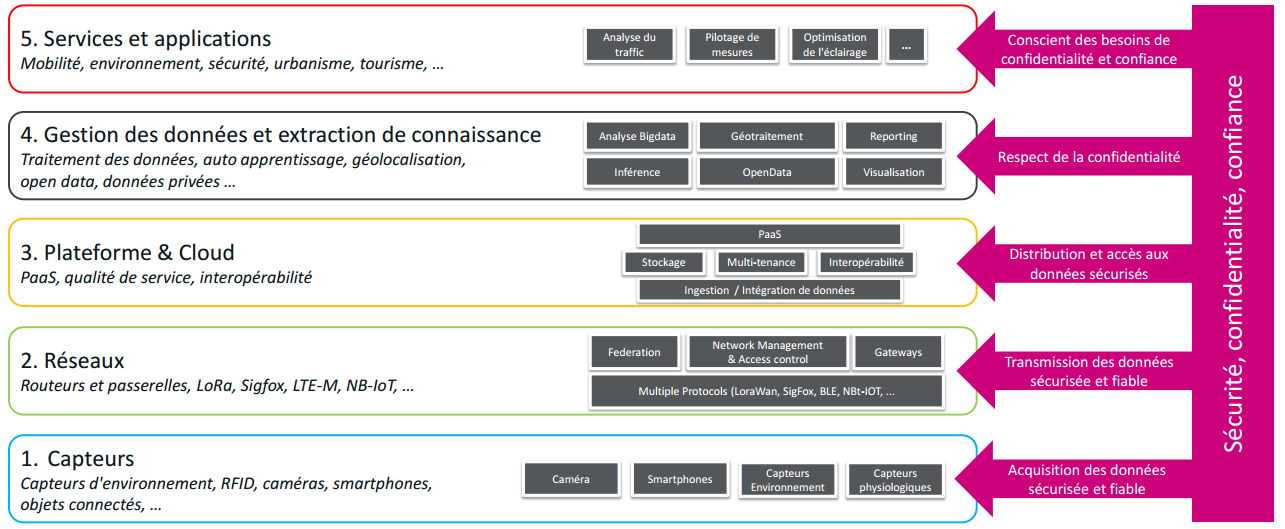
\includegraphics[width=1.0\textwidth]{Figures/StateOfTheArt/SmartCanton/architecture_smartcanton.png}
    \caption{Architecture générale du projet SmartCanton}
    \label{fig-architecture_smartcanton}
\end{figure}

Le POC peut être subdivisé en cinq couches interconnectées lesquelles sont détaillées sur la \cref{fig-architecture_smartcanton}. Le projet couvert par cette thèse de Master utilise principalement les deux premières de cette architecture. Le capteur est l'élément principal de ce travail, de même que son développement matériel et sa programmation. Un réseau doit ensuite être utilisé pour mettre à disposition les données capturées. Cette couche numéro 2 supporte ainsi plusieurs types de protocoles basés sur différentes technologies, tel que le LoRa, SigFox, etc. Dans le cadre de ce travail, l'accent porte sur la technologie LoRaWAN, couplée à la modulation LoRa. Parallèlement aux cinq couches de la \cref{fig-architecture_smartcanton}, on constate la présence de trois termes: Sécurité, Confidentialité et Confiance. Ceux-ci sont primordiaux dans les systèmes IoT modernes.

\begin{figure}[ht!]
    \centering
    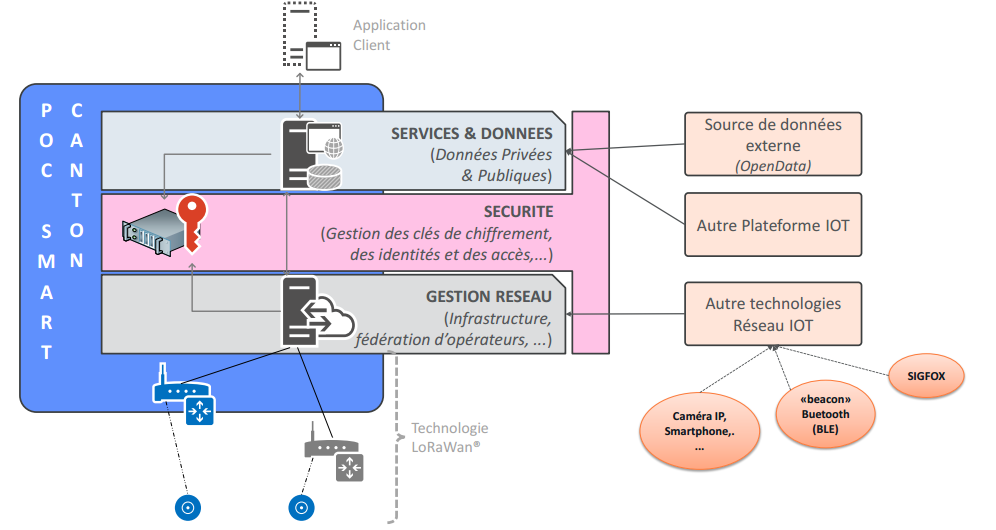
\includegraphics[width=0.9\textwidth]{Figures/StateOfTheArt/SmartCanton/infrastructure_smartcanton.png}
    \caption{Infrastructure LoRa du SmartCanton}
    \label{fig-infrastructure_smartcanton}
\end{figure}

La \cref{fig-infrastructure_smartcanton} expose la situation d'un point de vue plus appliqué à un réseau LoRaWAN. Les ronds bleu sur l'images correspondent aux périphériques LoRaWAN qui souhaitent transférer leurs données. Sur la même image, deux \textit{gateways} LoRaWAN différentes sont illustrées. Les raisons liées à cette différentiation sont exposés en \cref{sec-stateoftheart_smartcanton_federation}.


\subsection{Sécurité}


Le POC a exploré en détail les problématiques liées à la sécurité, tout particulièrement celles liées à la technologie LoRaWAN. Un \textit{Hardware Security Module} (HSM) (visible sur la \cref{fig-infrastructure_smartcanton}) a été intégré au coeur de la sécurité du SmartCanton. La sécurité utilisée au travers d'un réseau LoRaWAN est décrite à la \cref{sec-security_lorawan}. Celle spécifique au SmartCanton est quant à elle explorée à la \cref{sec-smartcanton_security}.



\subsection{Mise à disposition des données}


L'accès au données générées par les capteurs s'effectue à l'aide d'une infrastructure FIWARE\footnote{\url{https://www.fiware.org/}}. Cette plateforme a été développée dans le cadre du vaste projet Horizon 2020\footnote{\url{https://ec.europa.eu/programmes/horizon2020/}}, financé en partie par l'Union Européenne. 
L'environnement de FI-Ware est composé de plusieurs modules communicant entre eux à l'aide d'un protocole standardisé nommé NGSI. L'intégralité des composants de FI-Ware sont open-sources, prodiguant ainsi une liberté pour toute entité souhaitant implémenter une infrastructure complète.
Le but de ce projet est de proposer une plateforme intégralement open-source pour les besoin des \textit{smart technologies}. 

\subsection{Fédération d'opérateurs}
\label{sec-stateoftheart_smartcanton_federation}

Le POC SmartCanton utilise, grâce à un partenariat, une partie des infrastructures LoRa du réseau des Services Industriels de Genève\footnote{\url{https://www.sig-ge.ch/}} (SIG) et de l'entreprise Orbiwise\footnote{\url{https://www.orbiwise.com/home}}. Le but de cette collaboration est de couvrir au maximum le canton de Genève à l'aide des réseaux déjà existants.
Le \textit{roaming} des réseaux LoRaWAN ne sera couvert qu'avec l'arrivée de la nouvelle spécification LoRaWAN 1.1 (cf. \cref{sec-protocols_lorawan_spec_1_1} pour des informations supplémentaires sur le \textit{roaming}). Celle-ci ne dispose, à l'heure actuelle, d'aucun périphérique ou réseau d'opérateurs compatible.
Le concept de fédération des réseaux a donc du être mis en place dans le POC afin de récupérer des requêtes provenant de différents réseaux. La \cref{fig-federation_network} illustre les chemins d'accès disponibles depuis plusieurs opérateurs (Swisscom, SIG, Orbiwise et DGSI) qui, lorsqu'ils reçoivent des données d'un périphérique inconnu à leur propre réseau, peuvent rediriger les données vers la plateforme centralisée de la DGSI. Les divers composants illustrés sur ce diagramme (ex. \textit{Network Server}, \textit{Join Server}, etc.) sont explorés à la \cref{sec-protocols_lorawan}.



\begin{figure}[ht!]
    \centering
    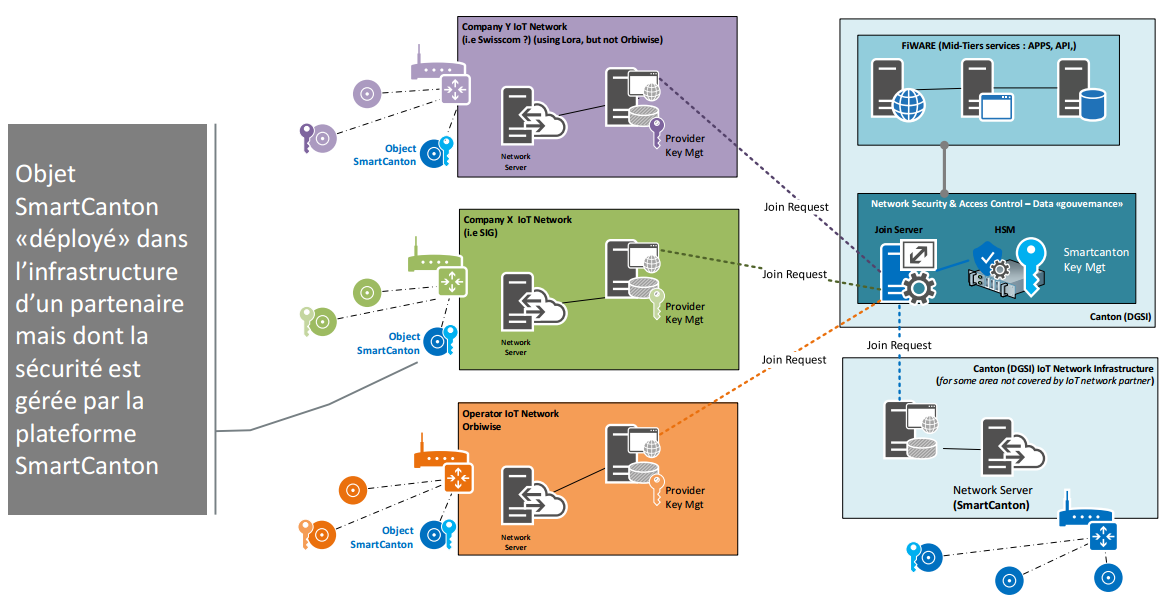
\includegraphics[width=1.0\textwidth]{Figures/StateOfTheArt/SmartCanton/federation_network.png}
    \caption{Fédération des réseaux}
    \label{fig-federation_network}
\end{figure}








